\section{Simulace a testování}

V této kapitole popíšu průběh simulací zaměřených na získání dat pro vyvážení herních mechanik a určení optimálních parametrů jednotek, budov a herního pole. V simulacích budu využívat konkrétní scénáře a také metodu Monte Carlo pro získání robustních dat.

\subsection{Cíle simulací}

Hlavními cíli těchto simulací je:

\begin{itemize}
\item Systematicky testovat atributy jednotek, produkci budov a ceny herních prvků v různých scénářích.
\item Nalézt vyvážené nastavení herních parametrů, kde žádný prvek není výrazně dominantní nebo zbytečný.
\item Analyzovat charakteristiky generovaného herního pole v závislosti na jeho parametrech.
\end{itemize}

\subsection{Metriky pro sběr dat a analýzu}

Pro sběr dat a analýzu v těchto simulacích se zaměřím na následující metriky v rámci jednotlivých testovaných scénářů:

\begin{itemize}
    \item \textbf{Živé jednotky (kolo):} Počet živých jednotek daného typu patřících danému hráči na konci kola.
    \item \textbf{Způsobené poškození (kolo):} Celkové nominální poškození, které jednotky daného typu patřící danému hráči způsobily v daném kole.
    \item \textbf{Reálně způsobené poškození (kolo):} Celkové skutečné poškození, které jednotky daného typu patřící danému hráči způsobily v daném kole, s ohledem na obranu cíle a terénní modifikátory.
    \item \textbf{Utržené poškození (kolo):} Celkové poškození, které jednotky daného typu patřící danému hráči utrpěly v daném kole.
    \item \textbf{Počet útoků (kolo):} Celkový počet útoků provedených jednotkami daného typu patřícími danému hráči v daném kole. Pomáhá pochopit aktivitu jednotek v boji.
    \item \textbf{Počet protiútoků (kolo):} Celkový počet protiútoků provedených jednotkami daného typu patřícími danému hráči v daném kole. Zaznamenává dodatečnou bojovou aktivitu.
    \item \textbf{Vítězství:} Který hráč vyhrál simulaci
    \item \textbf{Míra přežití jednotek (výsledek simulace):} Procento jednotek daného typu, které přežily celý střet.
    \item \textbf{Poškození (výsledek simulace):} Celkové poškození způsobené jednotkou daného typu během celého střetu.
    \item \textbf{Zranění (výsledek simulace):} Celkové poškození, které jednotka daného typu utrpěla během celého střetu.
    \item \textbf{Poměr ztrát (výsledek simulace):} Poměr mezi celkovým způsobeným poškozením a celkovým utrženým poškozením pro každou stranu v daném scénáři, nebo poměr počtu ztracených jednotek.
    \item \textbf{Počet kol (výsledek simulace):} Celkový počet kol, po kterých hra skončila.
    \item \textbf{Ekonomická efektivita (výsledek simulace):} Poměr mezi investovanými surovinami (náklady na jednotky) a dosaženými výsledky (např. celkové způsobené poškození).
\end{itemize}

\section{Teorie simulace}

Při provádění simulací budu využívat přístup podobný Monte Carlo metodě. Tato metoda spočívá v opakovaném náhodném vzorkování a simulaci s cílem získat statisticky robustní odhady chování komplexních systémů. 

V kontextu této práce to znamená, že jednotlivé testovací scénáře a celkové herní simulace budou spouštěny mnohokrát s potenciálně mírně odlišnými počátečními podmínkami (zejména v pozdějších fázích s náhodně generovanými mapami a prvkem náhody v rozhodování AI), abych získal průměrné výsledky a posoudil stabilitu a vyváženost herních mechanismů.

\subsection{Fáze 1: Testování vyváženosti jednotek a ekonomických parametrů v izolovaných scénářích}

V této fázi se zaměřím na testování jednotlivých typů jednotek proti sobě v kontrolovaných bojových situacích a zároveň budu zkoumat vliv cen jednotek a produkce surovin na jejich efektivitu.

\begin{itemize}
    \item \textbf{Scénáře 1v1:} Budu simulovat souboje mezi dvěma jednotkami různých typů (např. bojovník vs. lučištník) se stejnou nebo podobnou cenou.
    \item \textbf{Scénáře "armáda proti armádě":} Budu simulovat střety mezi menšími skupinami jednotek (např. 3 bojovníci vs. 2 lučištníci a 1 bojovník) se srovnatelnou celkovou cenou.
\end{itemize}

V rámci těchto scénářů mohu simulovat, jak rychlost získávání surovin ovlivňuje schopnost hráčů nasazovat jednotky v různých typech střetů.
Budu analyzovat, jak cena jednotky ovlivňuje její výkonnost v boji a její ekonomickou návratnost v kontextu verbování.

Na základě výsledků budu upravovat atributy a ceny jednotek a produkci budov a testovat upravené verze v nových scénářích.

\subsection{Fáze 2: Testování náhodného herního pole}

V této fázi se zaměřím na analýzu charakteristik generovaného herního pole v závislosti na parametrech generování mapy. Budu testovat různé kombinace parametrů, jako je velikost mapy, škálování Perlinova šumu a prahové hodnoty pro definici jednotlivých typů terénu. Pro každé nastavení budu provádět opakované generování map a sbírat následující statistiky:

\begin{itemize}
\item \textbf{Existence cesty mezi základnami:} Pro každou vygenerovanou mapu zjistím, zda existuje alespoň jedna průchodná cesta mezi počátečními pozicemi základen (předpokládám pevně dané startovní pozice pro účely tohoto testování).
\item \textbf{Délka nejkratší cesty mezi základnami:} Pokud cesta existuje, vypočítám délku nejkratší cesty (například pomocí algoritmu A* nebo Dijkstrova algoritmu s ohodnocením políček podle typu terénu).
\item \textbf{Existence "snadné" cesty (bez hor):} Zjistím, jak často existuje cesta mezi základnami, která neprochází přes horský terén ('H').
\item \textbf{Poměr zastoupení jednotlivých typů terénu:} Pro každou vygenerovanou mapu spočítám procentuální zastoupení jednotlivých typů terénu (voda 'V', pláně 'P', les 'L', hory 'H').
\end{itemize}

Cílem této fáze je identifikovat parametry generování map, které vedou k herním polím s vhodnými charakteristikami z hlediska průchodnosti, strategické hloubky (dané rozložením terénu) a potenciálu pro interakci mezi hráči.

\subsection{Fáze 3: Testování v celkových herních simulacích na náhodně generovaných mapách}

V této fázi se vrátím k simulacím celých her na náhodně generovaných mapách s jednoduchou AI, s již předběžně vyladěnými parametry jednotek a produkce budov z Fáze 1 a s nastavením generování map z Fáze 2, které se ukázalo jako nejvhodnější.

\begin{itemize}
\item \textbf{Sledování celkové dynamiky hry:} Budu sledovat délku her, frekvenci interakcí mezi hráči a celkový průběh hry.
\item \textbf{Sbírání dat pro finální doladění:} Budu shromažďovat data o využití jednotek a budov, výsledcích střetů a ekonomickém vývoji hráčů v reálných herních podmínkách pro případné další úpravy parametrů.
\end{itemize}

\section{Simulace}
V plné hře bude možné koupit pouze jednotky Pracovník a Bojovník, které pak hráč s použitím budov bude moci vylepšovat. Tento mechanismus není v prototypu implementován takže se v rámci simulace budu muset spokojit s odlišnou cenou jednotek na různé úrovni.

% TODO: Obrázek evoluce jednotek

Typy jednotek a jejich arbitrárně vybrané atributy jsou vidět v tabulce \ref{tab:atributy_jednotek_otocena}. S těmito hodnotami začneme testovat jednotky proti sobě a upravovat jejich vlastnosti dokud nebudou podobně hodnotné jednotky vykazovat podobnou sílu.

\newpage

\begin{sidewaystable}[h!]
\centering
\begin{tabular}{|l|*{9}{c|}}
\hline
\textbf{Atribut} & \textbf{Bojovník} & \textbf{Válečník} & \textbf{Rytíř} & \textbf{Berserkr} & \textbf{Lučištník} & \textbf{Ostrostřelec} & \textbf{Lovec} & \textbf{Základna} \\
\hline
Rychlost & 3 & 3 & 2 & 4 & 3 & 2 & 5 & 0 \\
\hline
Dosah & 1 & 1 & 1 & 1 & 4 & 6 & 3 & 0 \\
\hline
Útok & 5 & 8 & 10 & 12 & 7 & 10 & 7 & 0 \\
\hline
Obrana & 3 & 5 & 7 & 2 & 2 & 1 & 2 & 0 \\
\hline
Životy & 10 & 15 & 30 & 20 & 10 & 10 & 14 & 50 \\
\hline
Cena (jidlo) & 10 & 60 & 120 & 70 & 15 & 80 & 60 & 0 \\
\hline
Cena (dřevo) & 2 & 30 & 50 & 40 & 15 & 60 & 40 & 0\\
\hline
Cena (kámen) & 0 & 0 & 30 & 0 & 0 & 40 & 0 & 0 \\
\hline
Cena/kolo (jidlo) & 2 & 3 & 4 & 4 & 2 & 4 & 3 & 0 \\
\hline
Cena/kolo (dřevo) & 0 & 0 & 0 & 0 & 1 & 2 & 1 & 0 \\
\hline
Cena/kolo (kámen) & 0 & 0 & 1 & 0 & 0 & 0 & 0 & 0 \\
\hline
\end{tabular}
\caption{Atributy jednotek pro začátek simulace}
\label{tab:atributy_jednotek_otocena}
\end{sidewaystable}

\newpage


\subsection{Fáze 1: Základní vyvážení (1v1):}

V této fázi se zaměřím na testování jednotlivých typů jednotek proti sobě v kontrolovaných bojových situacích. 

Počáteční podmínky jsou známé a stálé a absence náhody v rozhodování AI to znamená, že výsledek každé jednotlivé simulace daného scénáře je vždy stejné, bude počet opakování snížen na deset. To slouží k ověření konzistence a zachycení případných anomálií, aniž by docházelo ke zbytečným výpočetním nárokům.

\paragraph{Mapy:}
\begin{itemize}
    \item \textbf{Rovná linie}
        \begin{itemize}
            \item \textbf{Mapa:} Linie (15 polí typu 'P' - pláně).
            \item \textbf{Umístění jednotek:} Jednotky budou začínat na opačných stranách linie (0, 0) a (14, 0).
            \item \textbf{Očekávané efekty a cíle:} Tento scénář testuje přímí souboj dvou jednotek bez možnosti manévrování nebo využití terénu. Cílem je porovnat jednotky v přímém boji bez manévrování.
        \end{itemize}
    \item \textbf{Rovina (velká otevřená plocha)}
        \begin{itemize}
            \item \textbf{Mapa:} Rovina (velká obdélníková mapa, 15x15 polí typu 'P' - pláně).
            \item \textbf{Umístění jednotek:} Jednotky budou začínat v opačných rozích (0, 0) a (14, 14).
            \item \textbf{Očekávané efekty a cíle:} Zvětšení celkové plochy poskytne prostor pro manévrování a ustupování.  Bude zde potřeba pohyb ve více směrech ne jen dopředu, což může mít vliv na efektivitu jednotek v boji. Cílem je zjisti zda otevřený prostor ovlivní výsledky.
        \end{itemize}
    \item \textbf{Pohoří (s horami uprostřed)}
        \begin{itemize}
            \item \textbf{Mapa:} Pohoří (obdélníková mapa, 15x15 s horami 'H' rozdělujícími mapu napůl oblepenými lesy).
            \item \textbf{Umístění jednotek:} Jednotky budou začínat v opačných rozích (0, 0) a (14, 14).
            \item \textbf{Očekávané efekty a cíle:} Horský terén ('H') modifikuje obranu jednotek stojících na něm (+2 obrana), zároveň ale také zásadně zpomaluje pohyb. To může mít zásadní dopad na souboj. Cílem je kvantifikovat, jak moc terén ovlivňuje balanc souboje.
        \end{itemize}
\end{itemize}

\subsubsection{Válečník vs. Lučištník}

Tento duel představuje souboj dvou základních archetypů jednotek po prvním vylepšení, z nichž se dále odvíjí celá evoluční větev jednotek. Cílem je posoudit, jak se odlišné atributy Válečníka (vyšší obrana a životy, kontaktní boj) a Lučištníka (dálkový útok, mobilita a schopnost ústupu) projeví na různých typech terénu. Očekáváme, že na rovinatých mapách s dostatkem prostoru bude Lučištník moci efektivněji využít manévrování, zatímco na lineární mapě bude souboj přímější a Válečník by mohl mít výhodu. Horský terén by pak měl výrazně zvýhodnit Lučištníka díky svým obranným bonusům a vlivu na pohyb.


\paragraph{Rovná linie}~ \newline

\textbf{Počáteční atributy:}
\begin{itemize}
\item \textbf{Jednotka A (Válečník):} \\ Útok:~8, Obrana:~5, Životy:~15, Rychlost:~3, Dosah:~1, \\ Cena (jídlo/dřevo/kámen):~60/30/0
\item \textbf{Jednotka B (Lučištník):} \\ Útok:~7, Obrana:~2, Životy:~10, Rychlost:~3, Dosah:~4, \\ Cena (jídlo/dřevo/kámen):~15/15/0
\end{itemize}

\textbf{Výsledky simulace (agregace 10 simulací):}
\begin{itemize}
\item \textbf{Poměr vítězství:} Válečník: 100\% simulací, Lučištník: 0\% simulací.
\item \textbf{Průměrný počet kol:} 4 kola
\item \textbf{Průměrné způsobené poškození za kolo (Válečník):} 3.00
\item \textbf{Průměrné způsobené poškození za kolo (Lučištník):} 1.50
\item \textbf{Průměrné utržené poškození za kolo (Válečník):} 1.50
\item \textbf{Průměrné utržené poškození za kolo (Lučištník):} 3.00
\item \textbf{Průměrný počet útoků za kolo (Válečník):} 0.50
\item \textbf{Průměrný počet protiútoků za kolo (Válečník):} 0.00
\item \textbf{Průměrný počet útoků za kolo (Lučištník):} 0.50
\item \textbf{Průměrný počet protiútoků za kolo (Lučištník):} 0.25
\item \textbf{Průměrná míra přežití (Válečník):} 100.00\%
\item \textbf{Průměrná míra přežití (Lučištník):} 0.00\%
\end{itemize}

\begin{figure}
  \centering      % vycentrovat
  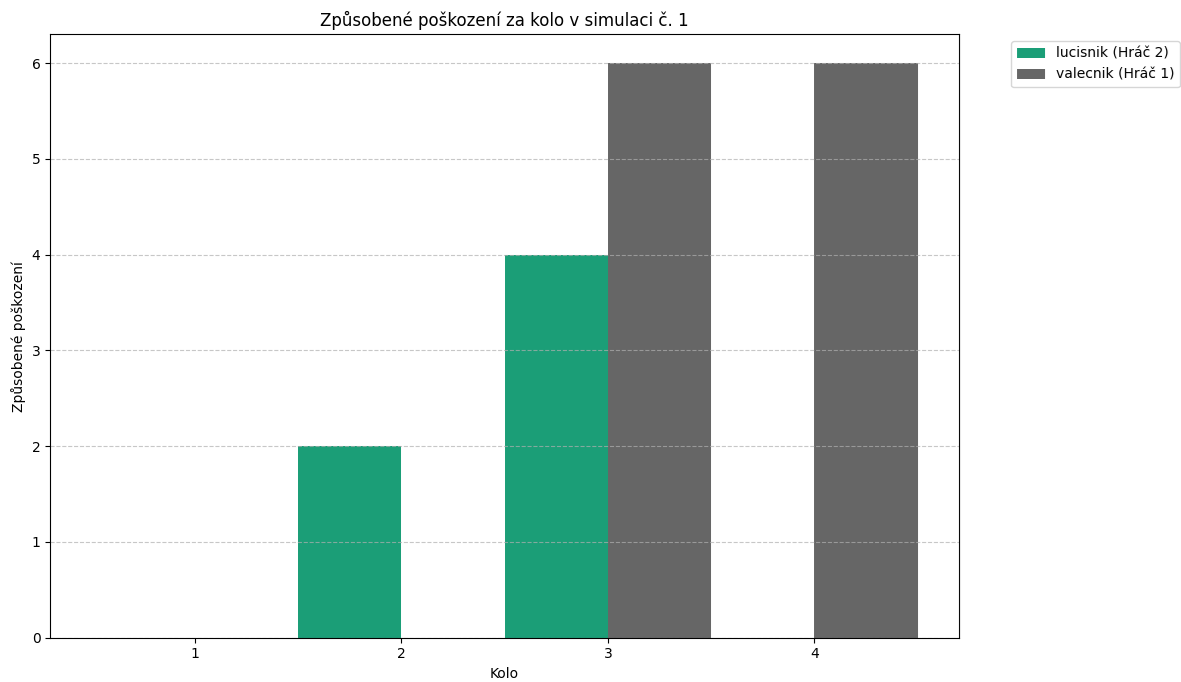
\includegraphics[scale=0.5]{obr/graf_valVSluc_linie_damage.png} % soubor + měřítko (scale)
  \caption{Graf poškození které jednotky způsobili v každém kole simulace} % popis obrázku
  \label{graf_valVSluc_linie_damage} % definice odkazu na obrázek (pro \ref{})
\end{figure}

\begin{figure}
  \centering      % vycentrovat
  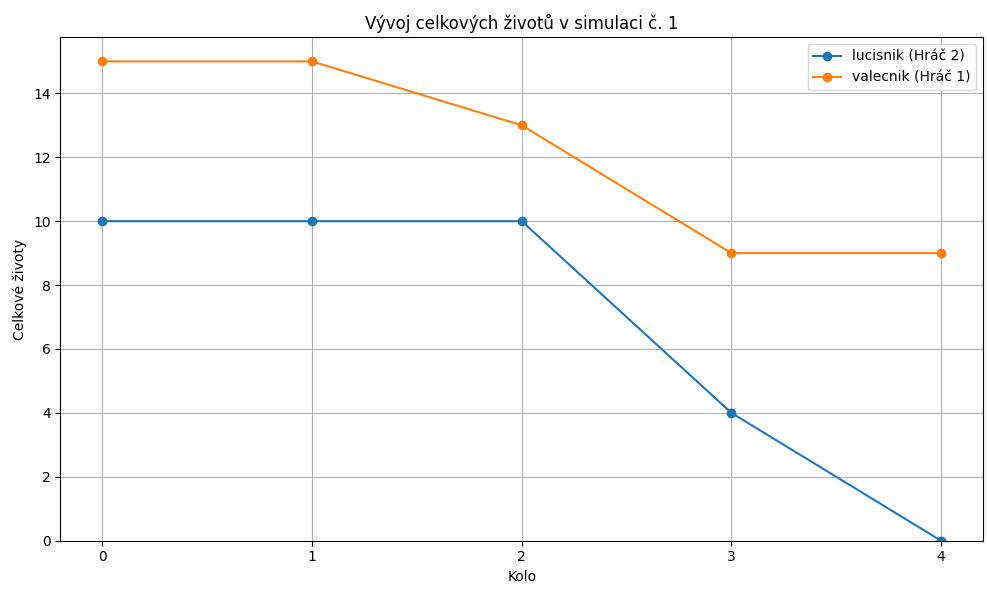
\includegraphics[scale=0.5]{obr/graf_valVSluc_linie_HP.png} % soubor + měřítko (scale)
  \caption{Graf životů jednotek v průběhu simulace} % popis obrázku
  \label{graf_valVSluc_linie_HP} % definice odkazu na obrázek (pro \ref{})
\end{figure}

\textbf{Analýza dat a interpretace:}

Na mapě Rovná linie, kde dochází k přímému střetu bez možnosti manévrování, se jasně ukázala \textbf{dominance Válečníka}, který zvítězil během průměrně 4 kol. Válečník způsobil průměrně 3.00 poškození za kolo a útočil s frekvencí 0.50 útoků za kolo, zatímco Lučištník způsobil 1.50 poškození za kolo se stejnou frekvencí útoků 0.50 za kolo. Lučištník navíc zaznamenal průměrně 0.25 protiútoků za kolo, což znamená, že poškození způsobil vícekrát než válečník. Zároveň je z obrázku \ref{graf_valVSluc_linie_HP} vidět, že válečník na konci neztratil ani polovinu svých životů.

Z toho je vidět, že útočná síla lučištníka je oproti obraně válečníka příliš malá, ačkoliv provedl více útoků, způsobil výrazně menší poškození. Tedy buď je potřeba snížit obranu válečníka, nebo zvýšit útok lučištníka.

\textbf{Navrhované úpravy atributů a zdůvodnění:}

Pro dosažení lepší vyváženosti v přímém souboji a zvýšení relevantnosti Lučištníka zkusím tyto úpravy a uvidím jak vyplyne souboj:

\begin{itemize}
    \item \textbf{Lučištník:}
    \begin{itemize}
        \item \textbf{Útok:} Zvýšení ze 7 na \textbf{8}.
        \item \textbf{Obrana:} Zvýšení z 2 na \textbf{3}.
        \item \textbf{Zdůvodnění:} Zvýšením útoku se Lučištník vyrovná Válečníkovi v základním poškození, což by mělo vést k efektivnějšímu snižování Válečníkových životů. Mírné navýšení obrany pak Lučištníkovi poskytne drobnou, ale potenciálně klíčovou výhodu pro přežití jednoho dalšího kola, což mu umožní způsobit více celkového poškození.
    \end{itemize}
    \item \textbf{Válečník:}
    \begin{itemize}
        \item \textbf{Obrana:} Snížení z 5 na \textbf{4}.
        \item \textbf{Zdůvodnění:} Snížení obrany Válečníka zvýší poškození, které obdrží od Lučištníka. To by mělo vést k rychlejšímu průběhu souboje z pohledu Válečníka a celkově vyrovnanějšímu střetu.
    \end{itemize}
\end{itemize}

\paragraph{Ověření úprav na mapě Rovná linie:}~ \newline

Po provedení navržených úprav jsem zopakoval simulaci na Linii.

\textbf{Nové výsledky simulace:}
\begin{itemize}
\item \textbf{Poměr vítězství:} Válečník: 100\% simulací, Lučištník: 0\% simulací.
\item \textbf{Průměrný počet kol:} 4 kola.
\item \textbf{Průměrné způsobené poškození za kolo (Válečník):} 2.50
\item \textbf{Průměrné způsobené poškození za kolo (Lučištník):} 3.00
\item \textbf{Průměrná míra přežití (Válečník):} 100.00\%
\item \textbf{Průměrná míra přežití (Lučištník):} 0.00\%
\end{itemize}

\begin{figure}
  \centering      % vycentrovat
  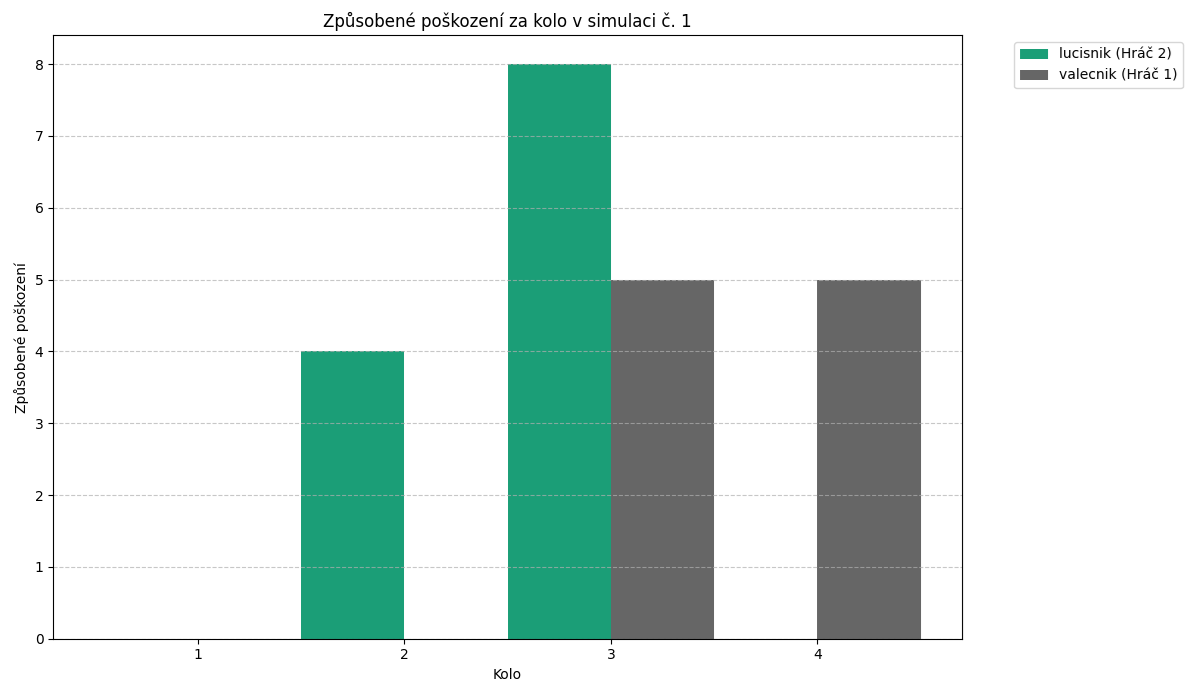
\includegraphics[scale=0.5]{obr/graf_valVSluc_linie_damage2.png} % soubor + měřítko (scale)
  \caption{Graf poškození které jednotky způsobili v každém kole simulace} % popis obrázku
  \label{graf_valVSluc_linie_damage2} % definice odkazu na obrázek (pro \ref{})
\end{figure}

\begin{figure}
  \centering      % vycentrovat
  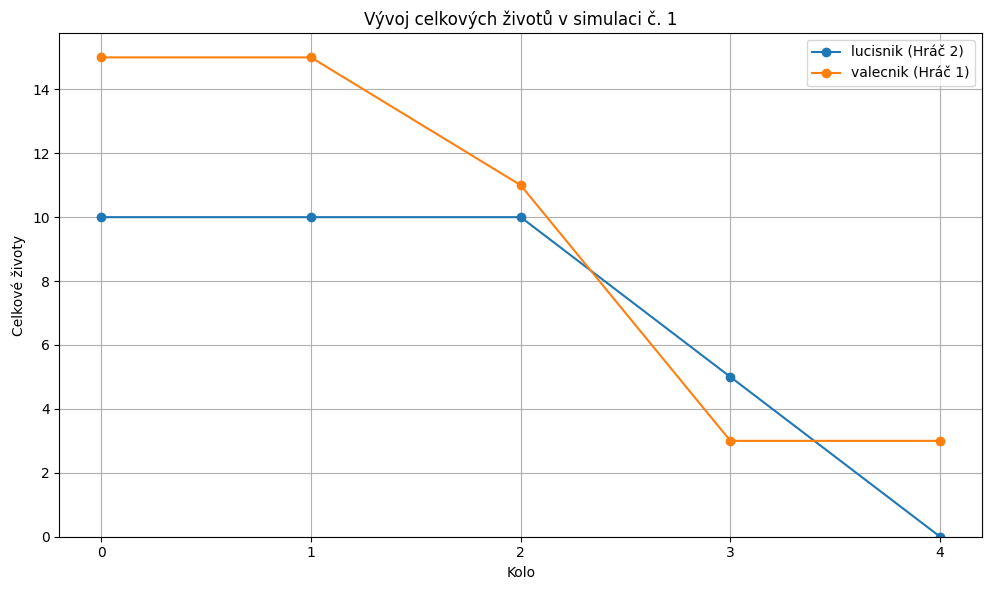
\includegraphics[scale=0.5]{obr/graf_valVSluc_linie_HP2.png} % soubor + měřítko (scale)
  \caption{Graf životů jednotek v průběhu simulace} % popis obrázku
  \label{graf_valVSluc_linie_HP2} % definice odkazu na obrázek (pro \ref{})
\end{figure}

Ačkoliv Válečník stále vyhrává všechny simulace, data ukazují jasné známky zlepšení vyvážení. Lučištník nyní průměrně způsobuje více poškození za kolo (3.00) než Válečník (2.50), což je zásadní obrat oproti předchozím simulacím.

Z grafu \ref{graf_valVSluc_linie_HP2} průběhu životů je patrné, že souboj je nyní mnohem vyrovnanější. Válečník končí simulace s pouze čtyřmi životy, což je výrazně nižší hodnota než před úpravami. Graf poškození \ref{graf_valVSluc_linie_damage2} navíc potvrdil, že ve druhém kole Lučištník skutečně způsobil větší poškození než Válečník, což demonstruje jeho zvýšenou útočnou efektivitu v klíčových momentech boje.

Tyto výsledky potvrzují, že provedené změny atributů měly zamýšlený dopad na dynamiku souboje a vedly k mnohem vyrovnanějšímu průběhu, i když poměr vítězství zůstává stejný.

\paragraph{Rovina}~ \newline

\textbf{Počáteční atributy:}
\begin{itemize}
\item \textbf{Jednotka A (Válečník):} Útok:~8, Obrana:~4, Životy:~15, Rychlost:~3, Dosah:~1, \\ Cena (jídlo/dřevo/kámen):~60/30/0
\item \textbf{Jednotka B (Lučištník):} Útok:~8, Obrana:~3, Životy:~10, Rychlost:~3, Dosah:~4, \\ Cena (jídlo/dřevo/kámen):~15/15/0
\end{itemize}

\textbf{Výsledky simulace (agregace 10 simulací):}
\begin{itemize}
\item \textbf{Poměr vítězství:} Válečník: 100\% simulací, Lučištník: 0\% simulací.
\item \textbf{Průměrný počet kol:} 10.00
\item \textbf{Průměrné celkové způsobené poškození za simulaci (Válečník):} 10.00
\item \textbf{Průměrné způsobené za kolo (Válečník):} 1.00
\item \textbf{Průměrný celkový počet útoků za simulaci (Válečník):} 2.00
\item \textbf{Průměrný celkový počet protiútoků za simulaci (Válečník):} 0.00
\item \textbf{Průměrná míra přežití (Válečník):} 100.00\%
\item \textbf{Průměrné celkové způsobené poškození za simulaci (Lučištník):} 12.00
\item \textbf{Průměrné způsobené za kolo (Lučištník):} 1.20
\item \textbf{Průměrný celkový počet útoků za simulaci (Lučištník):} 2.00
\item \textbf{Průměrný celkový počet protiútoků za simulaci (Lučištník):} 1.00
\item \textbf{Průměrná míra přežití (Lučištník):} 0.00\%
\end{itemize}

\begin{figure}
  \centering      % vycentrovat
  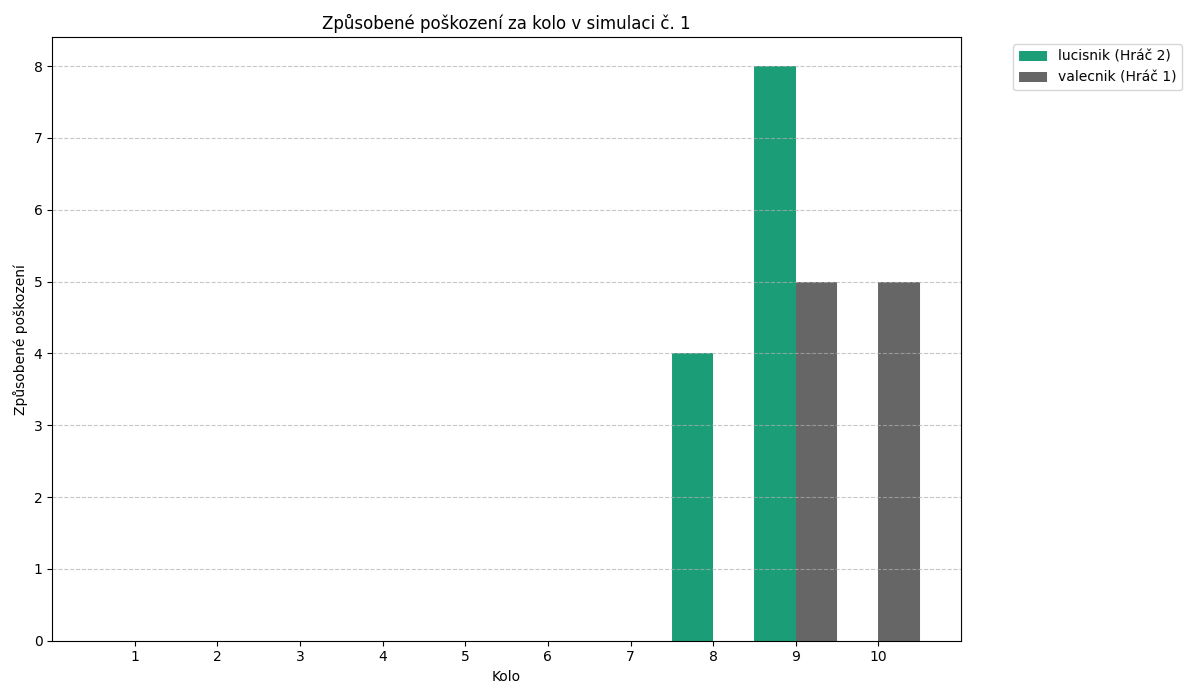
\includegraphics[scale=0.5]{obr/graf_valVSluc_flat_damage.png} % soubor + měřítko (scale)
  \caption{Graf poškození které jednotky způsobili v každém kole simulace} % popis obrázku
  \label{graf_valVSluc_flat_damage} % definice odkazu na obrázek (pro \ref{})
\end{figure}

\begin{figure}
  \centering      % vycentrovat
  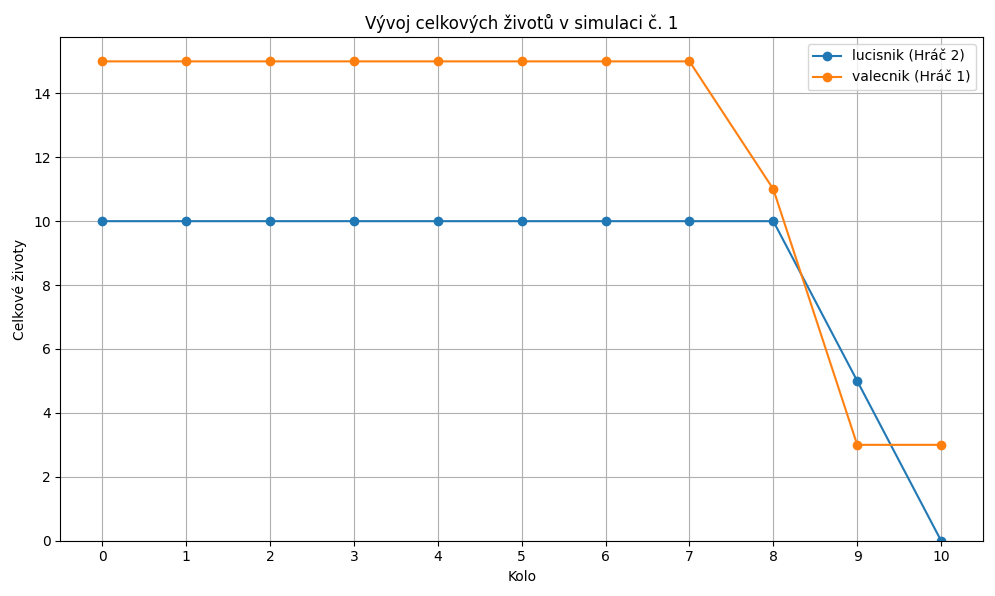
\includegraphics[scale=0.5]{obr/graf_valVSluc_flat_HP.png} % soubor + měřítko (scale)
  \caption{Graf životů jednotek v průběhu simulace} % popis obrázku
  \label{graf_valVSluc_flat_HP} % definice odkazu na obrázek (pro \ref{})
\end{figure}

\textbf{Analýza dat a interpretace:}

Průměrná délka souboje se oproti Linii prodloužila na 10 kol. Toto prodloužení souboje bylo zřejmě způsobeno tím, že jednotkám déle trvalo k sobě dojít, což jsem očekával, že bude zvýhodňovat lučištníka. K tomu nedošlo. Na grafech \ref{graf_valVSluc_flat_HP} a \ref{graf_valVSluc_flat_damage} je evidentně vidět, že jediná zásadní změna v tomto scénáři je delší doba, než se jednotky potkaly.

Tato simulace tedy nepřinesla žádné zásadní nové informace. Mohl bych zkusit lučištníka ještě trochu posílit, aby byl souboj ještě vyrovnanější, na druhou stranu je ale také pravda, že s lučištníkem se dají provádět strategické manévry, kterých prototypová AI není schopná, zkusím tedy atributy ponechat tak, jak jsou, a simulovat souboj v komplexnějším terénu.

\paragraph{Pohoří}~ \newline

\textbf{Počáteční atributy:}
\begin{itemize}
\item \textbf{Jednotka A (Válečník):} Útok:~8, Obrana:~4, Životy:~15, Rychlost:~3, Dosah:~1, \\ Cena (jídlo/dřevo/kámen):~60/30/0
\item \textbf{Jednotka B (Lučištník):} Útok:~8, Obrana:~3, Životy:~10, Rychlost:~3, Dosah:~4, \\ Cena (jídlo/dřevo/kámen):~15/15/0
\end{itemize}

\textbf{Výsledky simulace (agregace 10 simulací):}
\begin{itemize}
\item \textbf{Poměr vítězství:} Lučištník: 100\% simulací, Válečník: 0\% simulací.
\item \textbf{Průměrný počet kol:} 11.00
\item \textbf{Průměrné způsobené poškození za kolo (Válečník):} 0.55
\item \textbf{Průměrný počet útoků za kolo (Válečník):} 0.18
\item \textbf{Průměrná míra přežití (Válečník):} 0.00\%
\item \textbf{Průměrné způsobené poškození za kolo (Lučištník):} 1.45
\item \textbf{Průměrný počet útoků za kolo (Lučištník):} 0.55
\item \textbf{Průměrný počet protiútoků za kolo (Lučištník):} 0.18
\item \textbf{Průměrná míra přežití (Lučištník):} 100.00\%
\end{itemize}

\begin{figure}
  \centering      % vycentrovat
  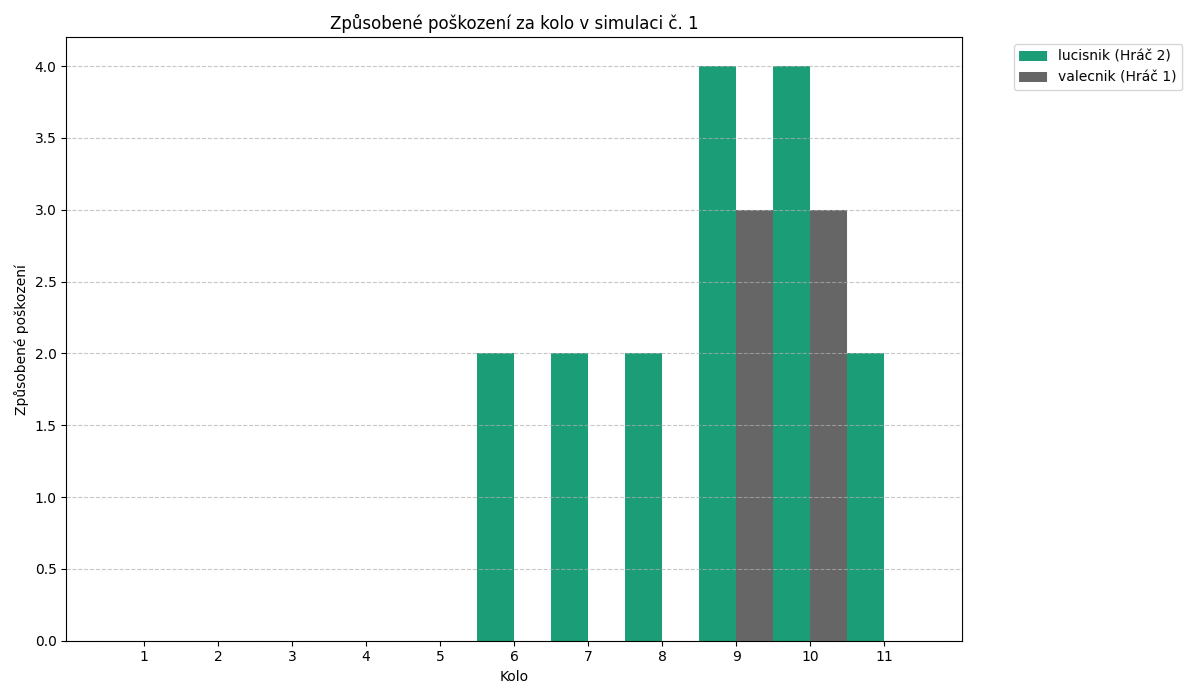
\includegraphics[scale=0.5]{obr/graf_valVSluc_nonflat_damage.png} % soubor + měřítko (scale)
  \caption{Graf poškození které jednotky způsobili v každém kole simulace} % popis obrázku
  \label{graf_valVSluc_nonflat_damage} % definice odkazu na obrázek (pro \ref{})
\end{figure}

\begin{figure}
  \centering      % vycentrovat
  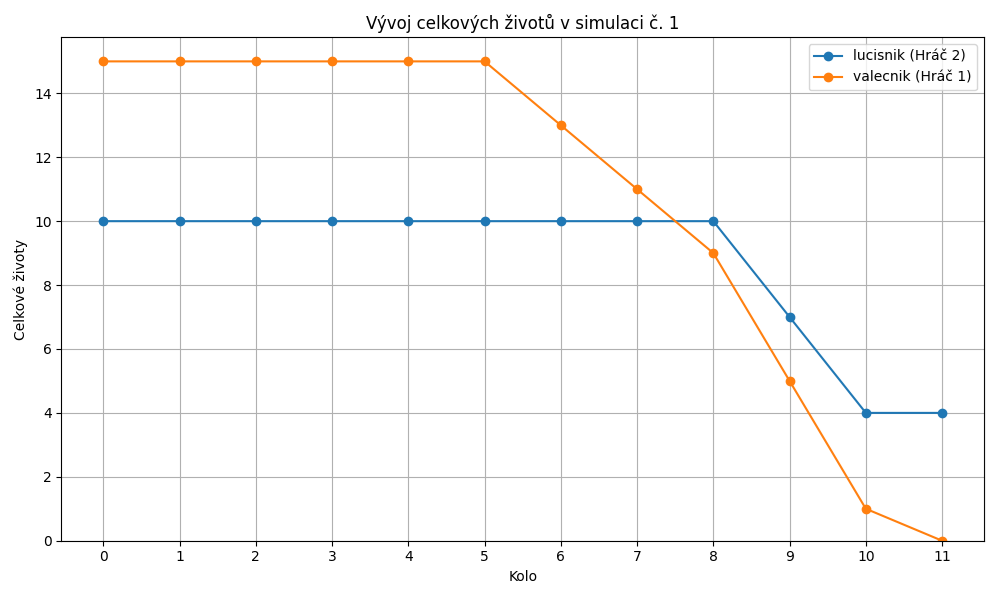
\includegraphics[scale=0.5]{obr/graf_valVSluc_nonflat_HP.png} % soubor + měřítko (scale)
  \caption{Graf životů jednotek v průběhu simulace} % popis obrázku
  \label{graf_valVSluc_nonflat_HP} % definice odkazu na obrázek (pro \ref{})
\end{figure}

\textbf{Analýza dat a interpretace:}

Průměrná délka souboje se prodloužila jen o jedno kolo, což je vzhledem k množství překážek překvapivé. Hory a lesy zpomalující pohyb válečníka, ale nepřekvapivě zásadně pomohli lučištníkovi způsobit dostatečné poškození, ačkoliv byl souboj těsný, lučištník tentokrát vyhrál.

V grafu poškození \ref{graf_valVSluc_nonflat_damage} je vidět, že celý souboj se odehrával v horách, kde je pohyb všech jednotek snížen na minimum, ale zároveň získávají jednotky bonus $+2$ k obraně. 

Z grafu životů \ref{graf_valVSluc_nonflat_HP} je pak vidět, že souboj byl těsný, lučištník už by další útok válečníka nepřežil, tedy prohlašuji jednotky za vyvážené.

\subsubsection{Rytíř vs. Berserkr}

\paragraph{Rovná linie}

\paragraph{Rovina}

\paragraph{Pohoří}

\subsubsection{Rytíř vs. Ostrostřelec}

\paragraph{Rovná linie}

\paragraph{Rovina}

\paragraph{Pohoří}

\subsubsection{Rytíř vs. Lovec}

\paragraph{Rovná linie}

\paragraph{Rovina}

\paragraph{Pohoří}

\subsubsection{Berserkr vs. Ostrostřelec}

\paragraph{Rovná linie}

\paragraph{Rovina}

\paragraph{Pohoří}

\subsubsection{Berserkr vs. Lovec}

\paragraph{Rovná linie}

\paragraph{Rovina}

\paragraph{Pohoří}

\subsubsection{Ostrostřelec vs. Lovec}

\paragraph{Rovná linie}

\paragraph{Rovina}

\paragraph{Pohoří}

\subsection{Fáze 1: Souboj více jednotek}
